\documentclass[12pt, a4paper]{article}
\usepackage{geometry}
\geometry{left=1.5 cm,right=1.5 cm,top=2.0 cm, bottom=2.0 cm}
\usepackage{amsmath}
\usepackage{graphicx}

\begin{document}

\title{Galaxy-Galaxy lensing}


\section{Theory}

\subsection{Distance}

Hubbule parameter:

\begin{align}
H^2 &= H_0^2[\frac{\Omega_r}{a^4}+\frac{\Omega_m}{a^3}-\frac{Kc^2}{a^2H_0^2}+\Omega_{\Lambda}] \\
&=H_0^2[\frac{\Omega_r}{a^4}+\frac{\Omega_m}{a^3}+\frac{1-\Omega_0}{a^2}+\Omega_{\Lambda}] 
\end{align}

Comving distance:

$$ dt = \frac{da}{\dot{a}} \Rightarrow -dw = \frac{cdt}{a} = \frac{cda}{a\dot{a}}=\frac{cda}{a^2H}$$

\begin{align}
\omega(z_1,z_2) &= \frac{c}{H_0}\int_{a(z_2)}^{a(z_1)} \frac{da}{\sqrt{a\Omega_m + a^2(1-\Omega_m -\Omega_\Lambda) + a^4\Omega_\Lambda}}, z_1 < z_2 \\
&= \frac{c}{H_0}\int_{z_1}^{z_2} \frac{dz}{\sqrt{(1+z)^3\Omega_m + (1+z)^2(1-\Omega_m -\Omega_\Lambda) + \Omega_\Lambda}}, z_1 < z_2 \\
&= \frac{c}{H_0}\alpha(z_1, z_2) 
\end{align}

The physical distance relates the angle to the size of a distant object is the angular diameter distance $D_A$. 

$$ D_A(z) = a(z)f_k(\omega(0,z))$$

The angular distance between $z_1$ and $z_2$ is

$$D_A(z_1, z_2) = a(z_2)f_k(\omega(z_1,z_2)) = \frac{c}{H_0}a(z_2)[\alpha(0, z_2) - \alpha(0, z_1)]$$

It is valid only for $\omega_k \geq 0 $ (see astro-ph/9905116 or Principles of Physical Cosmology pp 336–337, Peebles)


\subsection{Excess Surface Density}

\textbf{In comoving coordinate}
\begin{equation}
\Sigma_{crit}(z_L, z_S) = \frac{c^2}{4\pi G}\frac{D_A (z_S)}{D_A (z_L) D_A (z_L, z_S) (1+z_L)^2}
\end{equation}

\begin{align}
\frac{c^2}{4\pi G} 
&=\frac{c_0^2\times 10^{16}\ \rm{m^2\cdot s^{-2} }}{4\pi G_0\times 10^{-11}\  \rm{m^3\cdot s^{-2} \cdot Kg^{-1}}} \nonumber \\
&=\frac{c_0^2}{4\pi G_0}\times 10^{27} \ \rm{Kg \cdot m^{-1}} \nonumber \\
&=\frac{c_0^2 l_{pc}}{4\pi G_0}\times 10^{43} \ \rm{Kg \cdot pc^{-1}} \nonumber \\
&=\frac{c_0^2 l_{pc}}{4\pi G_0 m_{\odot}}\times 10^{13} \ \rm{M_{\odot} \cdot pc^{-1}} 
\end{align}

\begin{align}
&\frac{D_A (z_S)}{D_A (z_L) D_A (z_L, z_S) (1+z_L)^2} \nonumber \\
&=\frac{\omega(0,z_S)}{\omega(0,z_L)[\omega(0,z_S) - \omega(0,z_L)] (1+z_L)}\ \rm{h \cdot Mpc^{-1}} \\
&=\frac{\omega(0,z_S)}{\omega(0,z_L)[\omega(0,z_S) - \omega(0,z_L)] (1+z_L)}\times 10^{-6}\ \rm{h \cdot pc^{-1}} \\
&=\frac{\alpha(0,z_S)}{\alpha(0,z_L)[\alpha(0,z_S) - \alpha(0,z_L)] (1+z_L)}\frac{H_0}{c} \\
&=\frac{\alpha(0,z_S)}{\alpha(0,z_L)[\alpha(0,z_S) - \alpha(0,z_L)] (1+z_L)}\frac{100 \ \rm{h \cdot Km \cdot s^{-1} \cdot Mpc^{-1}}}{c_0\times 10^8 \ \rm{m \cdot s^{-1}}} \\
&=\frac{\alpha(0,z_S)}{\alpha(0,z_L)[\alpha(0,z_S) - \alpha(0,z_L)] (1+z_L)} \frac{1}{c_0} \times 10^{-9} \ \rm{h \cdot pc^{-1}}
\end{align}
\\

Using the \textbf{comoving distance} in calculation,
\begin{align}
\Sigma_{crit}(z_L, z_S) &= \frac{c_0^2 l_{pc}}{4\pi G_0 m_{\odot}}\times 10^{13} \ \rm{M_{\odot} \cdot pc^{-1}} \frac{\omega(0,z_S)}{\omega(0,z_L)[\omega(0,z_S) - \omega(0,z_L)] (1+z_L)}\times 10^{-6}\ \rm{h \cdot pc^{-1}} \nonumber\\
&=\frac{c_0^2 l_{pc}}{4\pi G_0 m_{\odot}}\frac{\omega(0,z_S)}{\omega(0,z_L)[\omega(0,z_S) - \omega(0,z_L)] (1+z_L)}\times 10^7 \ \rm{h \cdot M_{\odot}\cdot pc^{-2}} \nonumber\\
&=\frac{\omega(0,z_S)}{\omega(0,z_L)[\omega(0,z_S) - \omega(0,z_L)] (1+z_L)}\times 1662895.2081868195 \ \rm{h \cdot M_{\odot} \cdot pc^{-2}}
\end{align}
\\

Using the \textbf{integrate part of comoving distance} instead of distance itself in calculation,
\begin{align}
\Sigma_{crit}(z_L, z_S) &= \frac{c_0^2 l_{pc}}{4\pi G_0 m_{\odot}}\times 10^{13} \ \rm{M_{\odot} \cdot pc^{-1}} \frac{\alpha(0,z_S)}{\alpha(0,z_L)[\alpha(0,z_S) - \alpha(0,z_L)] (1+z_L)} \frac{1}{c_0} \times 10^{-9} \ \rm{h \cdot pc^{-1}} \nonumber \\
&=\frac{c_0 l_{pc}}{4\pi G_0 m_{\odot}}\frac{\alpha(0,z_S)}{\alpha(0,z_L)[\alpha(0,z_S) - \alpha(0,z_L)] (1+z_L)}\times 10^4 \ \rm{h \cdot M_{\odot}\cdot pc^{-2}} \nonumber\\
&=\frac{\alpha(0,z_S)}{\alpha(0,z_L)[\alpha(0,z_S) - \alpha(0,z_L)] (1+z_L)}\times 554.6821355281792 \ \rm{h \cdot M_{\odot} \cdot pc^{-2}}
\end{align}
\\



\noindent \textbf{In physical coordinate}
\begin{equation}
\Sigma_{crit}(z_L, z_S) = \frac{c^2}{4\pi G}\frac{D_A (z_S)}{D_A (z_L) D_A (z_L, z_S)}
\end{equation}
\begin{align}
&\frac{D_A (z_S)}{D_A (z_L) D_A (z_L, z_S)} \nonumber \\
&=\frac{(1+z_L)\omega(0,z_S)}{\omega(0,z_L)[\omega(0,z_S) - \omega(0,z_L)]}\times 10^{-6}\ \rm{h \cdot pc^{-1}} \\
&=\frac{(1+z_L)\alpha(0,z_S)}{\alpha(0,z_L)[\alpha(0,z_S) - \alpha(0,z_L)]} \frac{1}{c_0} \times 10^{-9} \ \rm{h \cdot pc^{-1}}
\end{align}
\\

Using the \textbf{comoving distance} in calculation,
\begin{align}
\Sigma_{crit}(z_L, z_S) &= \frac{c_0^2 l_{pc}}{4\pi G_0 m_{\odot}}\times 10^{13} \ \rm{M_{\odot} \cdot pc^{-1}} \frac{(1+z_L)\omega(0,z_S)}{\omega(0,z_L)[\omega(0,z_S) - \omega(0,z_L)]}\times 10^{-6}\ \rm{h \cdot pc^{-1}} \nonumber\\
&=\frac{c_0^2 l_{pc}}{4\pi G_0 m_{\odot}}\frac{(1+z_L)\omega(0,z_S)}{\omega(0,z_L)[\omega(0,z_S) - \omega(0,z_L)]}\times 10^7 \ \rm{h \cdot M_{\odot}\cdot pc^{-2}} \nonumber\\
&=\frac{(1+z_L)\omega(0,z_S)}{\omega(0,z_L)[\omega(0,z_S) - \omega(0,z_L)]}\times 1662895.2081868195 \ \rm{h \cdot M_{\odot} \cdot pc^{-2}}
\end{align}
\\

Using the \textbf{integrate part of comoving distance} instead of distance itself in calculation,
\begin{align}
\Sigma_{crit}(z_L, z_S) &= \frac{c_0^2 l_{pc}}{4\pi G_0 m_{\odot}}\times 10^{13} \ \rm{M_{\odot} \cdot pc^{-1}} \frac{(1+z_L)\alpha(0,z_S)}{\alpha(0,z_L)[\alpha(0,z_S) - \alpha(0,z_L)]} \frac{1}{c_0} \times 10^{-9} \ \rm{h \cdot pc^{-1}} \nonumber \\
&=\frac{c_0 l_{pc}}{4\pi G_0 m_{\odot}}\frac{(1+z_L)\alpha(0,z_S)}{\alpha(0,z_L)[\alpha(0,z_S) - \alpha(0,z_L)]}\times 10^4 \ \rm{h \cdot M_{\odot}\cdot pc^{-2}} \nonumber\\
&=\frac{(1+z_L)\alpha(0,z_S)}{\alpha(0,z_L)[\alpha(0,z_S) - \alpha(0,z_L)]}\times 554.6821355281792 \ \rm{h \cdot M_{\odot} \cdot pc^{-2}}
\end{align}
\\

\begin{equation}
c_0 = 2.99\ 792\ 458; \quad  l_{pc} = 3.085\ 677\ 581; \quad m_{\odot} = 1.9885, \quad M_{\odot} = 1.9885\times 10^{30}\  \rm{Kg}; \quad G_0 = 6.67\ 408\ 313 \nonumber
\end{equation}


\subsection{Rotation}
To calculate the tangential shear or Excess Surface Density, one must rotate the ellipticity according the position angle definition in Figure \ref{rotation}. The position angle and the direction of rotation will be different in many papers.

\subsection{sphere}
\begin{figure}[h]
	\centering
	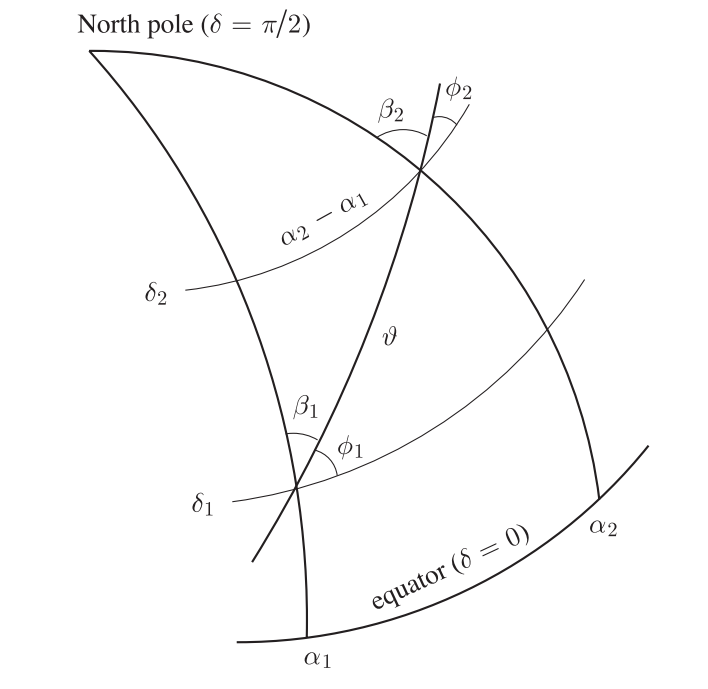
\includegraphics[width=0.5\textwidth]{sphere.PNG}
	\caption{Sphere}
	\label{sphere}
\end{figure}




\subsubsection{shear estimators rotation}
Rotation of shear:
\begin{align}
e_{+} = e_1 \cos 2\theta - e_2 \sin 2\theta \nonumber \\
e_{\times} = e_1 \sin 2\theta + e_2 \cos 2\theta \nonumber \\
\end{align}

\begin{figure}[h]
\centering
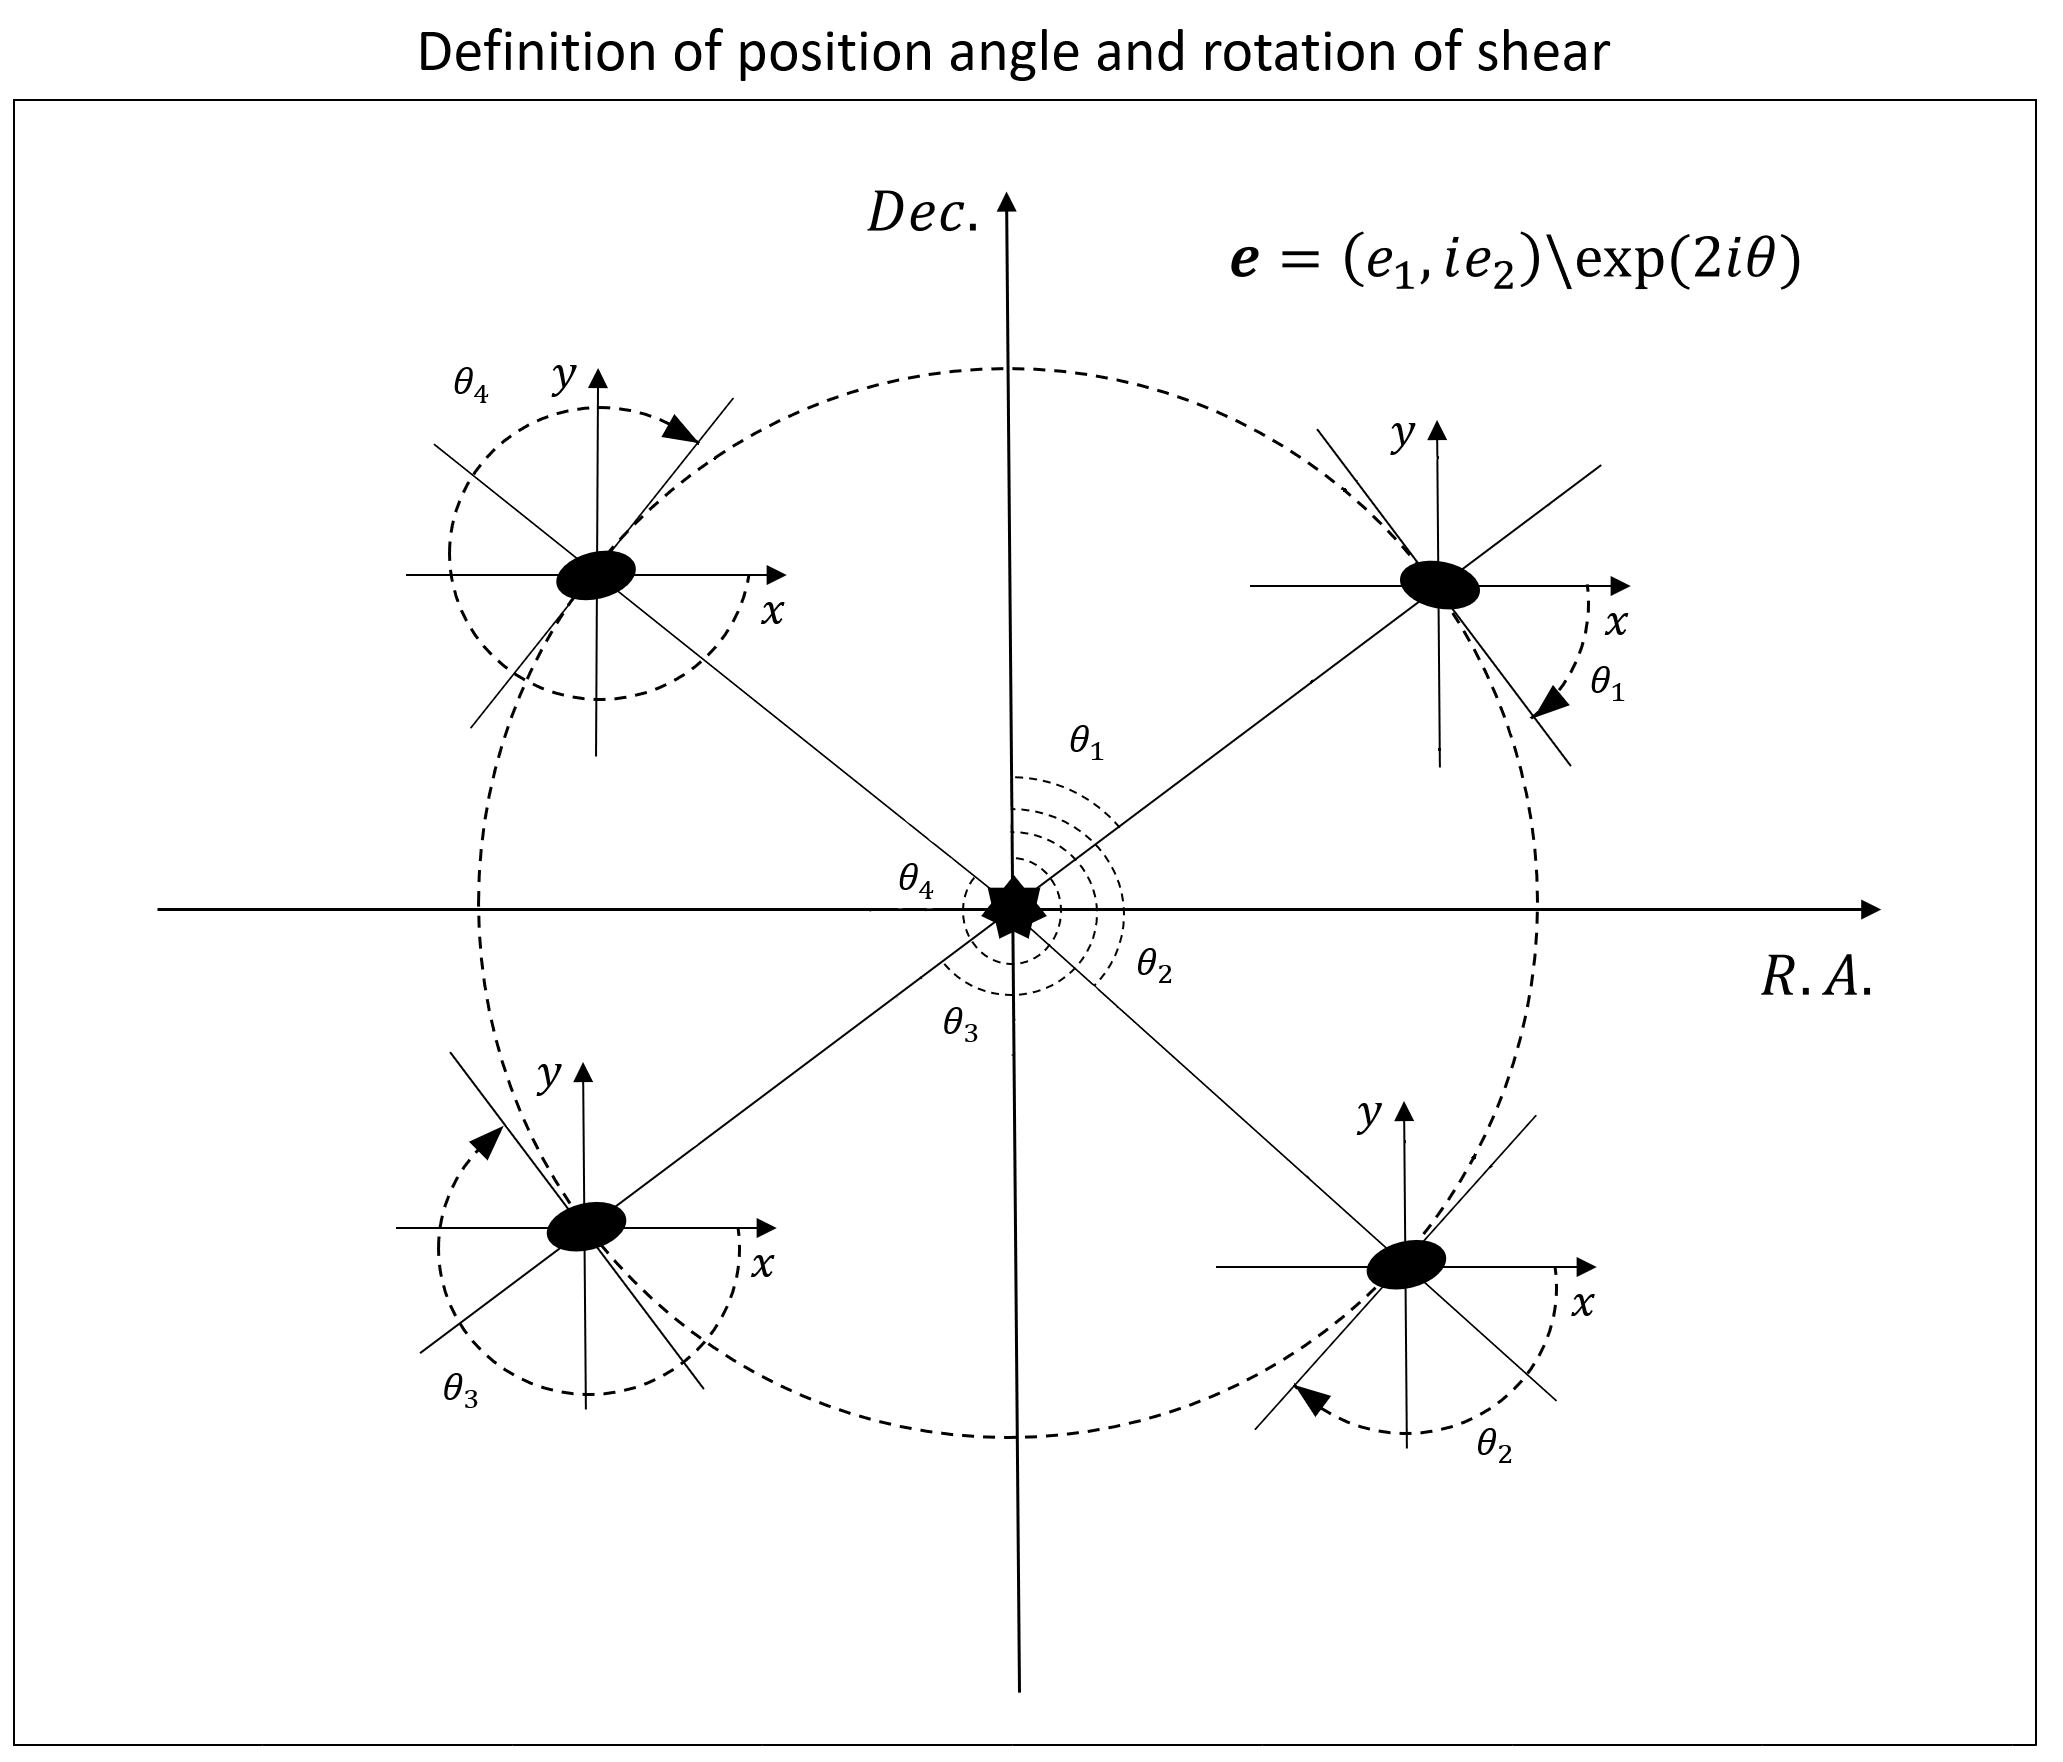
\includegraphics[width=0.8\textwidth]{rotation.png}
\caption{Rotation}
\label{rotation}
\end{figure}

The rotation of the shear estimator : $G_1$,$G_2$,$N$,$U$,$V$.
\begin{align} 
G_{+}+ iG_{\times} &= (G_1+iG_2) \exp (2i\phi) \\
G_{+} &= G_1\cos (2\phi)  - G_2\sin (2\phi) \\
G_{\times} &= G_1\sin (2\phi)  + G_2\cos (2\phi) \\
N &\rightarrow N \\
U^{\prime}+iV^{\prime} &= (U+iV)\exp (4i\phi) \\
U^{\prime} &= U\cos (4\phi)  - V\sin (4\phi) \\
V^{\prime} &= U\sin (4\phi)  + V\cos (4\phi) 
\end{align}
\\

\subsection{Parameters}
Mass of sun:
\begin{equation}
M_{\odot} = 1.9885 \times 10^{30} \rm{Kg},\quad m_{\odot} = 1.9885
\end{equation} 
%from [NASA](https://nssdc.gsfc.nasa.gov/planetary/factsheet/sunfact.html).


Gravitational constant:
\begin{equation}
G = 6.67\  408(31) \times 10^{-11} \ \rm{m^3 \cdot Kg^{-1}\cdot s^{-2}}
\end{equation}
%from [Mohr, Peter J., Newell, David B., Taylor, Barry N. (2015-07-21). "CODATA Recommended Values of the Fundamental Physical Constants: 2014". Reviews of Modern Physics. 88 (3): 035009.](https://journals.aps.org/rmp/pdf/10.1103/RevModPhys.88.035009)

Speed of light:
\begin{equation}
c = 299\  792\  458 \ \rm{m\cdot s^{-1}} = 2.99\  792\  458 \times 10^8 \ \rm{m\cdot s^{-1}}
\end{equation} 
%[idem.](https://journals.aps.org/rmp/pdf/10.1103/RevModPhys.88.035009)

\begin{equation}
1\  \rm{AU} = 149\  597\  870\  700 \ \rm{m} = 1.49\   597\   870\   700 \times 10^{11} \ \rm{m}
\end{equation}
%from [International Astronomical Union](https://www.iau.org/static/resolutions/IAU2012_English.pdf)

\begin{equation}
1 \ \rm{Persec} =  3.085\  677\  581 \times 10^{16} \ \rm{m}
\end{equation}



\subsection{NFW profile}
\begin{equation}
\rho(r)= \frac{\rho_s}{[\frac{r}{r_s}][1+\frac{r}{r_s}]^2}
\end{equation}
\section{How to...}
There two similar pipelines for \textbf{CFHT} and \textbf{Fourier\_Quad}.

Firstly, the distance should be calculated. ``\textbf{calculate\_co-distance.py}'' calculates the comoving distance $(Mpc/h)$ and the integrate part in the distance calculate for the final GGL calculation. 
The parameters should be specified in code. The data will be saved in a hdf5 file. The distances will be signed to the source catalog in ``\textbf{prepare\_background\_cata.py}''.

\noindent``\textbf{/OM0\_H0\_C}'' contains a array of $\Omega_{m0}$, $H_0$, and $C_0(\sim 2.9)$.

\noindent``\textbf{/Z}'' contains the redshifts ($0 \sim Z_{max}$).

\noindent``\textbf{/DISTANCE}'' contains the distances ($Mpc/h$).

\noindent``\textbf{/DISTANCE\_INTEG}'' the integrate part of the distance.

\subsection{CFHT catalog}

\subsubsection{Prepare data}
\textbf{1.} ``\textbf{add\_ODD\_Z\_B.py}'' adds \textbf{Z\_MIN}, \textbf{Z\_MAX}, and \textbf{ODDS} (from the .csv files) to the \textbf{CFHT} catalog for source selection.
It will create two new files (.hdf5 \& \_new.dat) that contains the added parameters.
\\ \hspace*{\fill} \\
\noindent The hdf5 file contains 3 arrays:

\noindent``\textbf{/data}'': the catalog with the 3 added parameters. The column: \emph{``RA  DEC  Flag  FLUX\_RADIUS  e1  e2  weight  fitclass   SNratio  MASK  Z\_B  m  c2  LP\_Mi  star\_flag  MAG\_i  \textbf{Z\_B\_MIN  Z\_B\_MAX  ODDS}}''. The last three are added.

\noindent``\textbf{/mask}'': it should be 1 for each source

\noindent``\textbf{/dRA\_dDEC}'': delta RA and delta DEC, they should be very small for each source ( $< 10^{-5}$)
\\ \hspace*{\fill} \\

\noindent\textbf{2.} Run ``\textbf{prepare\_background\_cata.py}'' in ``\textbf{collect}'' mode with MPI to stack the data from each field. It creates the ``\textbf{cfht\_cata.hdf5}'' in the parent directory of the one contain the field catalog. The data in $i$-th area will be in ``/w\_i'' in the .hdf5 file. \textbf{If the catalog file (cfht\_cata.hdf5) doesn't exist, run it firstly!} Before this step, \textbf{CFHT} catalog contains 19 ($0\sim 18$) columns. After this the 19'th \& 20'th column are the PZ data from Dong FY.
\\ \hspace*{\fill} \\

\noindent\textbf{3.} Run ``\textbf{prepare\_background\_cata.py}'' in ``\textbf{select}'' mode with CPU's as the same number as the area. The result will be in \textbf{cfht\_cata\_cut.hdf5}. The cutoff should be specified in the code. The program will create a few additional data for GGL calculation (see the code). At the end, the first thread will call ``add\_com\_dist (add\_com\_dist.cpp)'' to sign distance to the source.

\end{document}